\chapter{Global optimization scheme} \label{ch:scheme}
In Chapter 1, it is introduced that optimizing the stiffness of the coupling robot in the manufacturing process can improve the manufacturing accuracy of the workpiece. The comparison and analysis of optimization methods through Chapter 2, the choice of using particle swarm optimization method to improve the stiffness of physically coupled robots in the manufacturing process. This chapter presents the development of a global optimization scheme for enhancing stiffness.
\section{Machining Process} \label{sec:scheme:process}
\subsection{Machining Path} \label{subsec:sec:scheme:process:path}
Machining is a process in which a material is cut to a desired final shape and size by a controlled material-removal process. The three principal machining processes are classified as turning, drilling and milling. The machining path is the path through space that the tip of a cutting tool follows to produce the desired geometry of the workpiece. The physically coupled robots perform coordinated machining tasks. Various machining tasks, such as drilling and milling, can be implemented if tools are attached to the coupler. 
\subsubsection{Path generation} \label{subsubsec:subsec:sec:scheme:process:path: path generation}
The given machining path is converted according to the G-code. G-code is the most widely used computer numerical control (CNC) programming language \cite{cncs}. It is used mainly in computer-aided manufacturing to control automated machine tools and has many variants. Extensions and variations of G-code have been added independently by control manufacturers and machine tool manufacturers, and operators of a specific controller must be aware of the differences between each manufacturer's product. In CNC machining centers, the G-code is composed of the letter G and two digits and is used for the control of tool paths, i.e., the movement of each feed axis, such as linear or arc interpolation, feed control, offset and transformation of the origin of the coordinate system, setting of dimensional units, tool offset and compensation. \par
The machining path can be generated using a combination of lines and arcs as the basic elements according to the G-code introduction above \cite{dqt}. Each element has a starting phase (velocity from zero to a constant value) and an ending phase (velocity from a constant value to zero). The basic elements overlap in their transition phases so that a line can be smoothly connected to an arc with a continuous position and velocity \cite{dqt}. \par
A $\boldsymbol{timeframes} = (t_{i,j})_{n \times 4}$ can represent the relationship between a given machining path and time. $t_{i,1}$ represents the time value in the i-th element corresponding to a speed of zero in the starting phase, $t_{i,2}$ represents the time value in the i-th element corresponding to a speed of a constant value in the starting phase, $t_{i,3}$ represents the time value in the i-th element corresponding to a speed of a constant value in the ending phase and $t_{i,4}$ represents the time value in the i-th element corresponding to a speed of zero in the ending phase. n represents a machining path with n basic elements. $\boldsymbol{timeframes}$ can be shown as follows:
\begin{equation}
\boldsymbol{timeframes} = \begin{bmatrix} 
    t_{1,1} & \dots  & b_{1,4}\\
    \vdots & \ddots & \vdots\\
    b_{n,1} & \dots  & b_{n,4} 
    \end{bmatrix}
    \label{eq:tframe}
\end{equation}
According to the path characterization, there is a special relationship between $t_{i,3}$ and $t_{i+1,1}$, $t_{i,4}$ and $t_{i+1,2}$. As the acceleration phase corresponding to each element and the deceleration phase corresponding to the last element are fitted to the final machining path, the time values $t_{i,3}$ and $t_{i+1,1}$, $t_{i,4}$ and $t_{i+1,2}$ are averaged as the characteristic time points of the sampling points. Then, based on the matrix (\ref{eq:tframe}), the following vector $\boldsymbol{t_{\mathrm{characteristic}}}$ generated from the characteristic time points can be obtained. In the same way, this vector is the key data for the next step of data processing.
\begin{equation}
  \boldsymbol{t_{\mathrm{characteristic}}} =  \begin{bmatrix}
       t_{1,1} & \frac{t_{1,3}+t_{2,1}}{2} & \frac{t_{1,4}+t_{2,2}}{2} &  & \dots & \frac{t_{n-1,3}+t_{n,1}}{2} & \frac{t_{n-1,4}+t_{n,2}}{2} & t_{n,4} \end{bmatrix}^\top
       \label{eq:tcha}
\end{equation}
\subsection{Data Pre-processing} \label{subsec:sec:scheme:process:Data Pre-processing}
The challenge of enhancing stiffness is finding the stiffest configurations along the entire path, not at a single point. That means the coupled robot needs to move along a predefined machining path to ensure that the actual machining path matches the predefined path. The path is on the workpiece, and the workpiece can be placed freely in the space. In addition, evaluating and optimizing robots' configurations along a continuous machining path are time-consuming, so data pre-processing is needed to reduce the computation.
% \subsubsection{Choice of sampling method}\label{subsubsec:subsec:sec:scheme:process:Data Pre-processing:sampling method}
Data pre-processing, in other words, is the use of a sampling method to extract sample points. Commonly used sampling methods are equal distance sampling and equal time interval sampling. As the sampling methods listed previously do not consider information about the characteristics of the machining path, such as straight lines or curves, they increase the number of sampling points. Therefore, the more computational effort is required to complete the optimization process later. \par
In order to better take into account the feature information of the path points and to reduce the number of sampling points, resampling will be performed based on the above obtained time-dependent characteristic vector $\boldsymbol{t_{\mathrm{characteristic}}}$. The vector is shown as (\ref{eq:tcha}). \par
Firstly, introduce the resampling and its sampling process. The resampling is based on the data obtained from the previous matrix $\boldsymbol{t_{\mathrm{characteristic}}}$ relating to time, removing some unnecessary points to reduce the number of sampled points. \par
The resampling process is as follows:
\begin{itemize}
 \item \textbf{Step 1}: There is a series of points on the curve: $p_{0},p_{1}...p_{n-1},p_{n}$, as shown in
Figure \ref{fig:main:sampling1}. $p_{0}$ represents the path point under the time value corresponding to the first element of the vector $\boldsymbol{t_{\mathrm{characteristic}}}$, $p_{1}$ represents the second element, and so on. $p_{n}$ refers to the path point of the last element.
\item \textbf{Step 2}: Calculate the distance of $p_{1},p_{2}...p_{n-1}$ to the line $p_{0},p_{n}$ as shown in Figure \ref{fig:main:sampling2}.
\item \textbf{Step 3}: Find the maximum value of distance $p_{k}$, as shown in
Figure \ref{fig:main:sampling3}.
\item \textbf{Step 4}: If $p_{k}\leq d_\mathrm{tolerance}$, save $p_{0},p_{n}$ two points is sufficient. Else divide into two polylines at the point where $p_{k}$ is located and go to Step 2. $d_\mathrm{tolerance}$ is the required sampling tolerance.
\end{itemize}
\begin{figure}[h!]
\centering
\vspace{-1cm}
\setlength{\abovecaptionskip}{-1cm} 
\begin{minipage}[t]{0.48\textwidth}
\centering
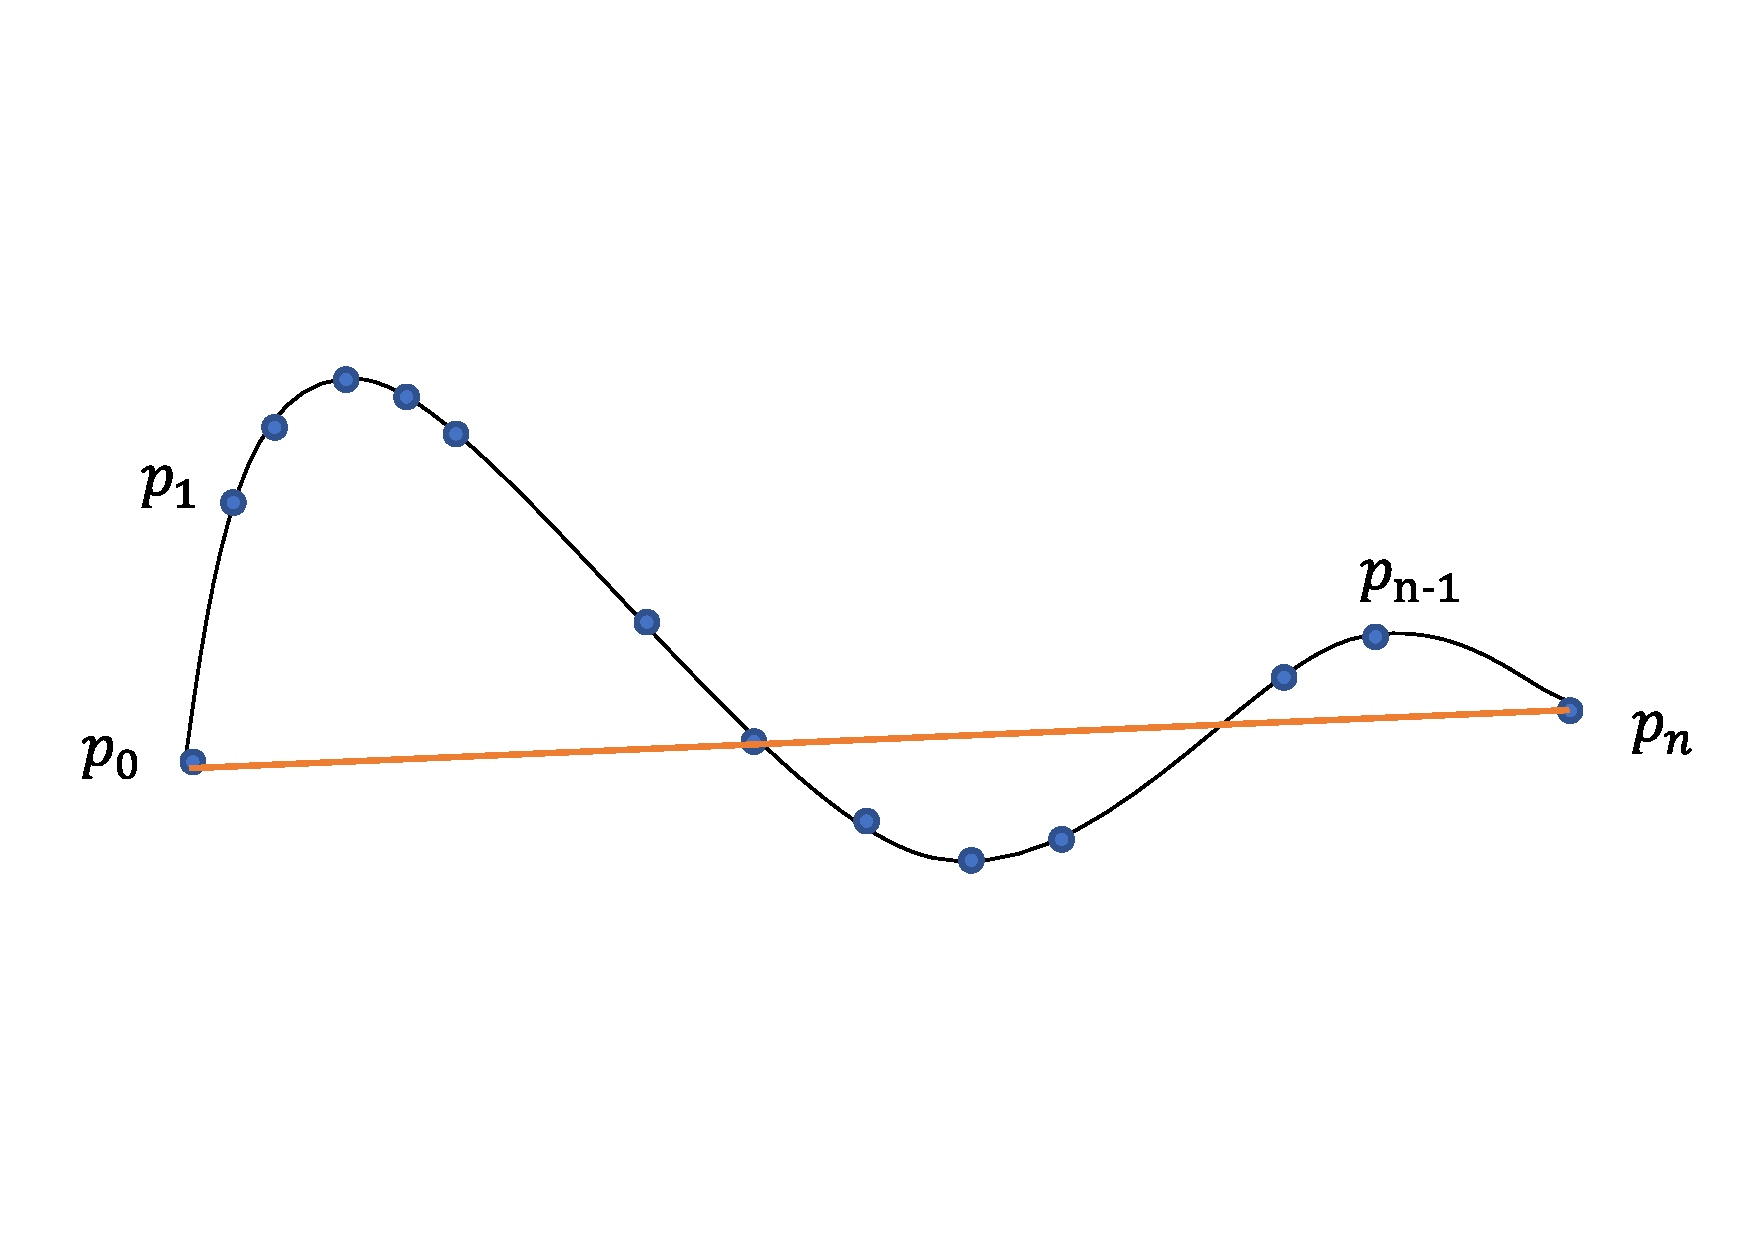
\includegraphics[width=6cm]{03_images/sampling_1.pdf}
\caption{Step 1}
\label{fig:main:sampling1}
\end{minipage}
\begin{minipage}[t]{0.48\textwidth}
\centering
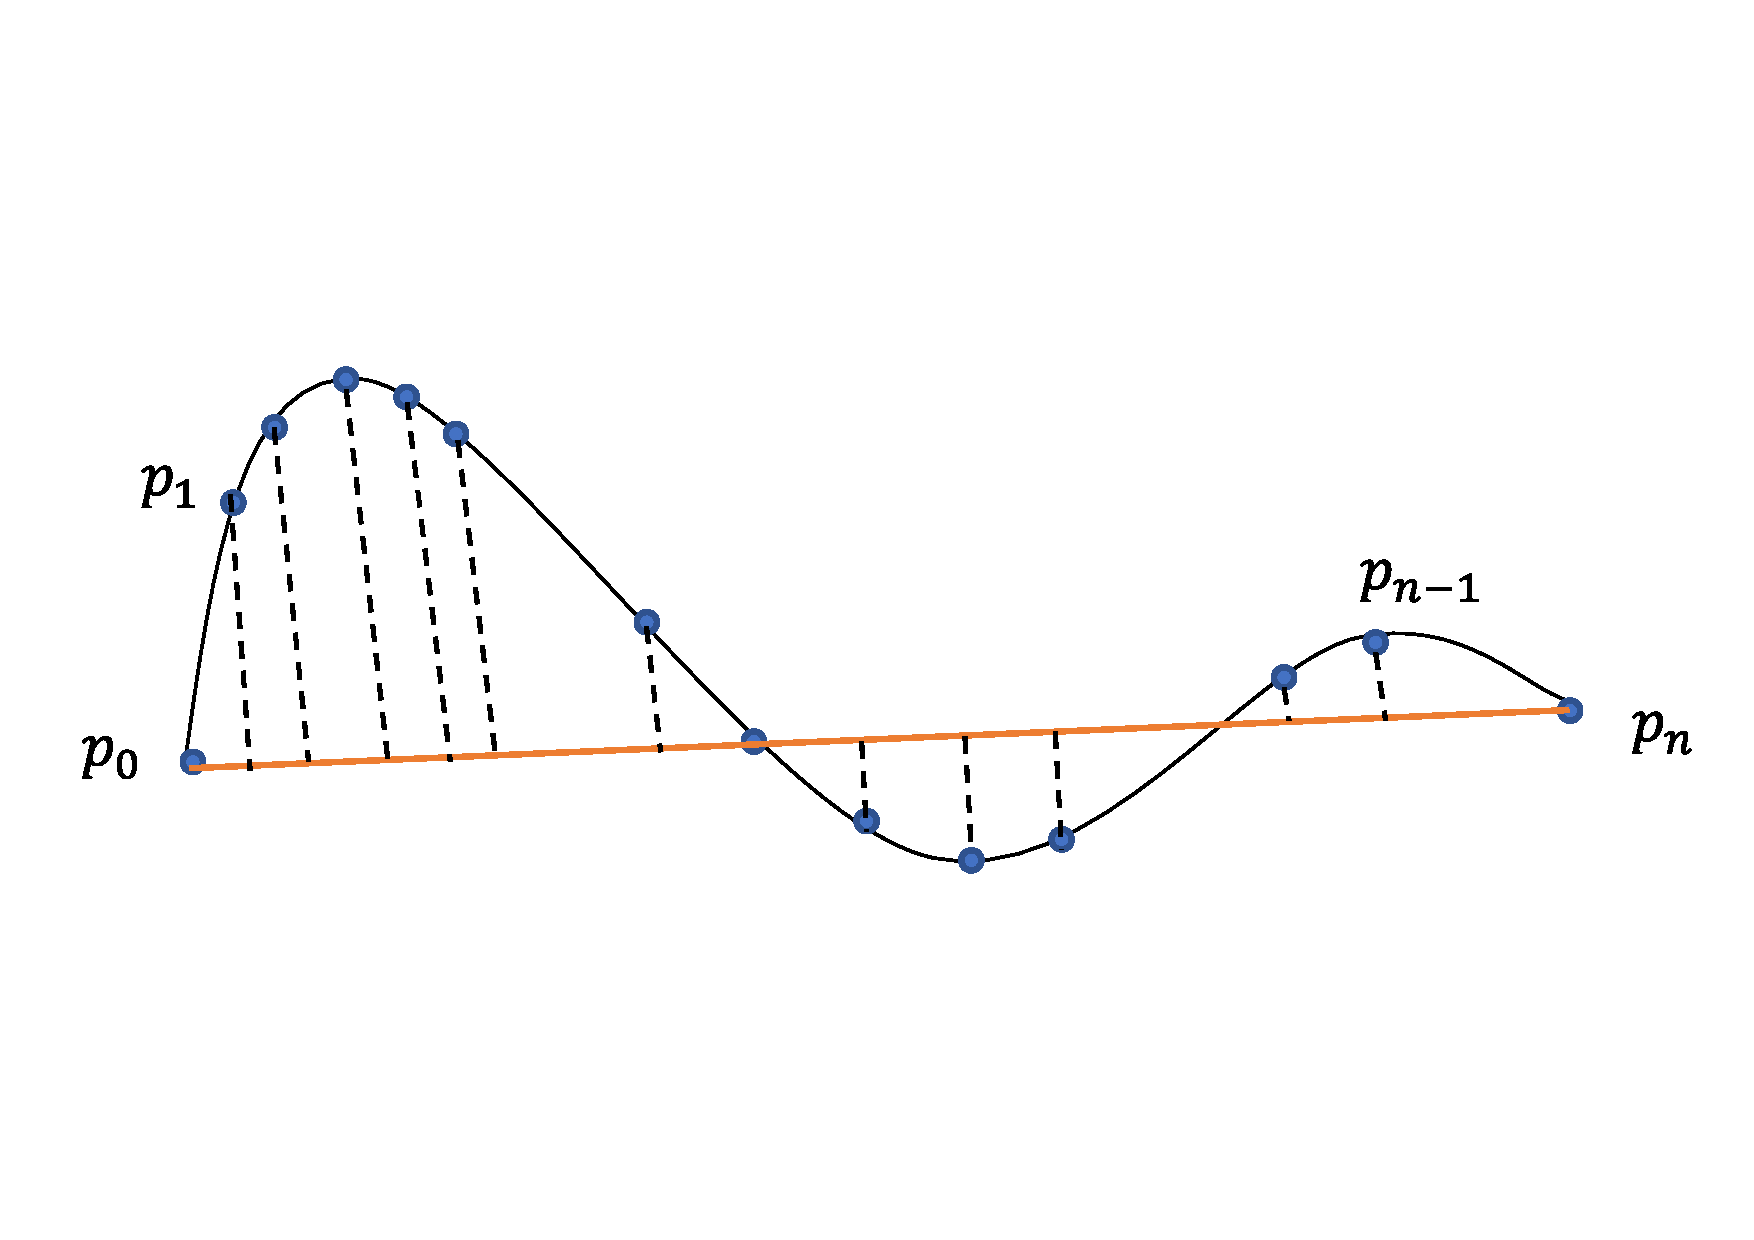
\includegraphics[width=6cm]{03_images/sampling_2.pdf}
\caption{Step 2}
\label{fig:main:sampling2}
\end{minipage}
\end{figure}
\begin{figure}[h!]
	\centering
        \vspace{-1.7cm}
        \setlength{\abovecaptionskip}{-1cm}
	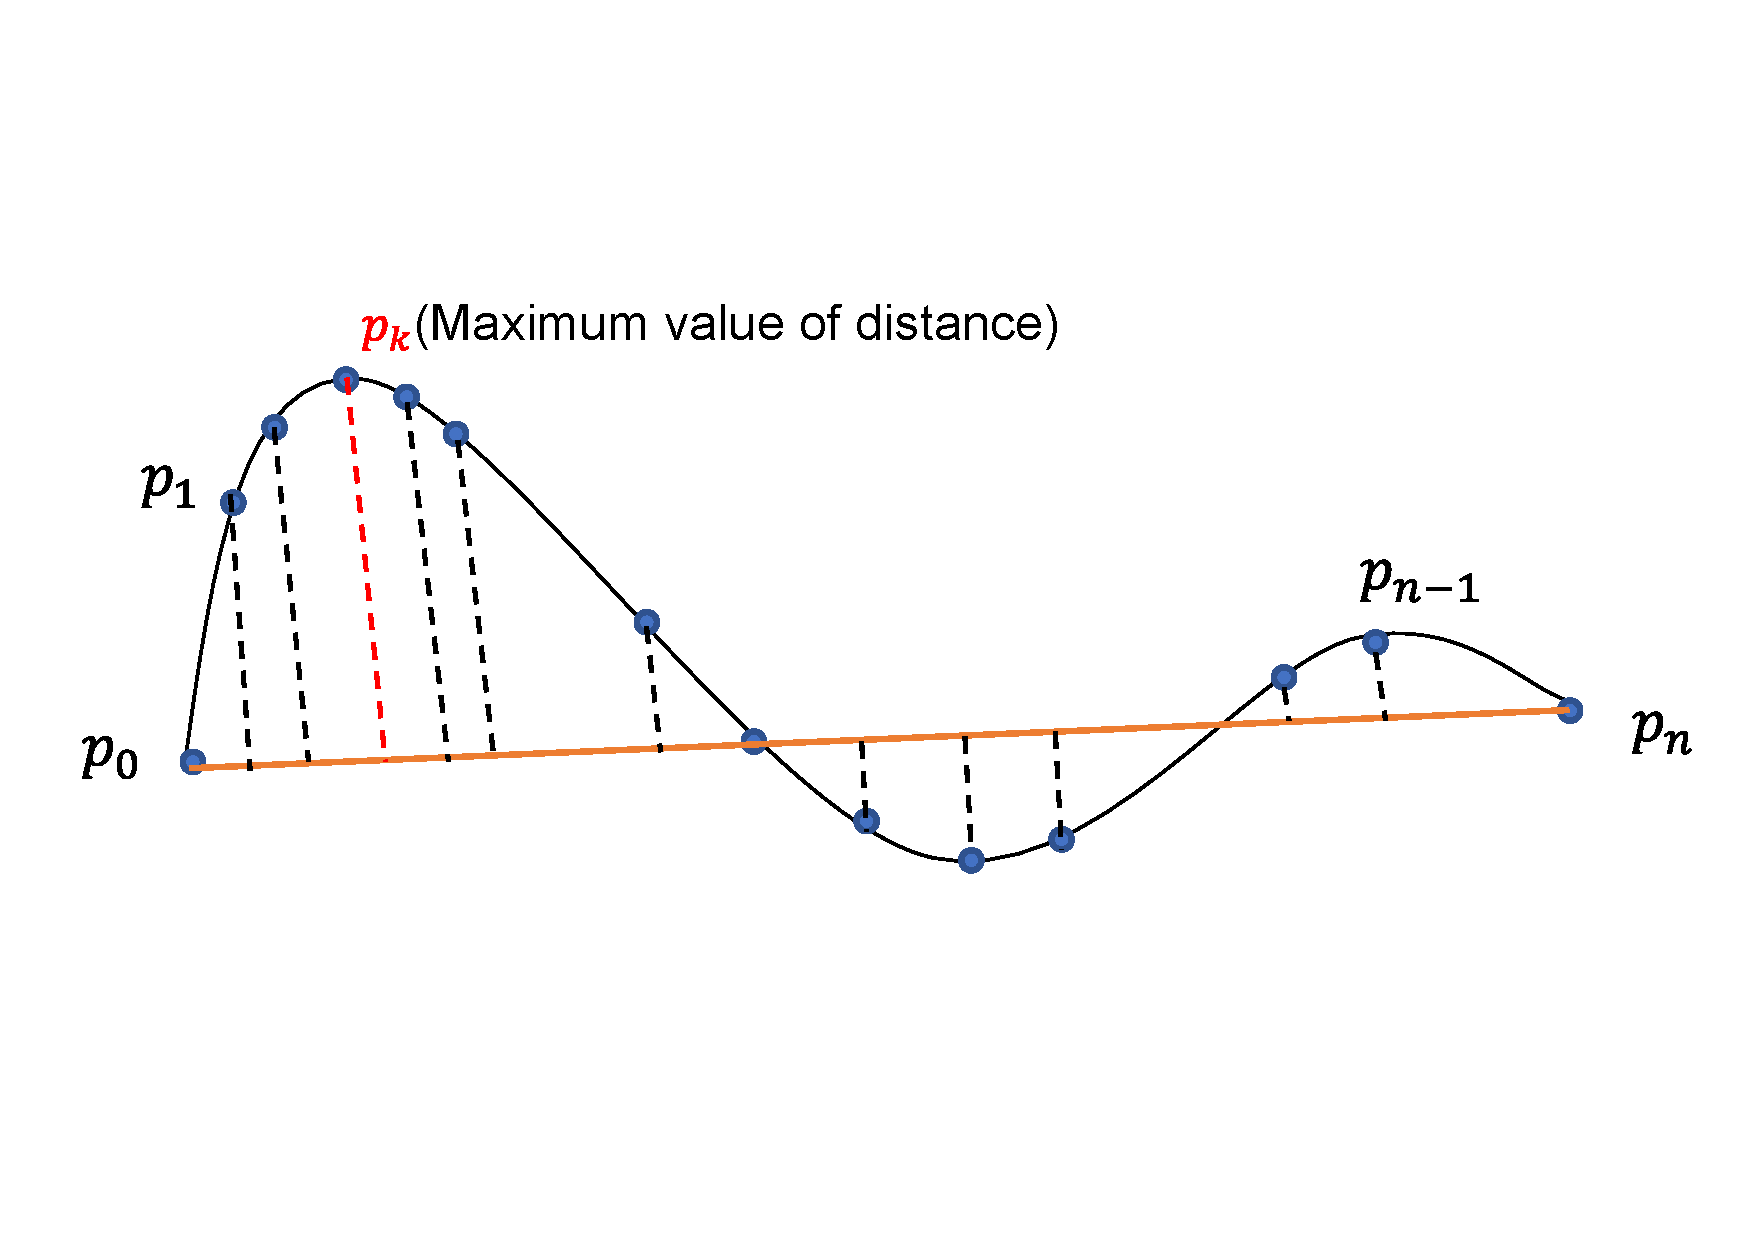
\includegraphics[width=6cm]{03_images/sampling_3.pdf}
	\caption{Step 3}
	\label{fig:main:sampling3}
\end{figure}
% \subsection{Acquisition of sampled points for machining path }\label{subsec:sec:Main:Pre-processing:sampled points}
Based on the introduction of the resampling steps, the following will explain how resampling is applied to the data pre-processing process.\par
Before applying resampling to the data pre-processing, it needs to be determined how step 2 above calculates the point-to-line distance as in equation (\ref{eq:cald}). 
\begin{equation}
   d_{i} = \frac{\left|(p_{i}-p_{0}) \times (p_{i}-p_{n})\right|}{\left|(p_{n}-p_{0})\right|} 
\label{eq:cald}
\end{equation}
$p_{i}$ represents a point apart from the first and last points on the path, $p_{0}$ represents the first point of the path, and $p_{n}$ represents the last point. \par
\begin{algorithm}
\SetAlgoLined
\caption{Resampling} \label{alg1} 
\KwData{The relationship between a given machining path and time: $\boldsymbol{timeframes} \in \mathbb{R}^{n\times4}$,\;
Time-dependent characteristic vector: $\boldsymbol{tcha}$,\;
Time corresponding to the start point of the currently analysed part of the machining path: $t_\mathrm{start}$, \;
Time corresponding to the end point of the currently analysed part of the machining path: $t_\mathrm{end}$, \;
Minimum value of the time interval between two points: $\epsilon$,\;
Sampling tolerance: $d_\mathrm{tolerance}$}
\KwResult{Matrix of the times corresponding to the sampled points after resampling: $\boldsymbol{sample_{\mathrm{path}}}$ }
$t_\mathrm{start}\gets \boldsymbol{tcha}_{1}$;\;
$t_\mathrm{end}\gets \boldsymbol{tcha}_{2}$;\;
$\boldsymbol{sample_{\mathrm{path}}} \gets \left[ \right]$;\;
\While{$\boldsymbol{tcha} \neq \varnothing $}{
    \eIf{$\boldsymbol{tcha}$ contains only one element}{
    Add $\boldsymbol{tcha}_{1}$ to the last element of the matrix $\boldsymbol{sample_{\mathrm{path}}}$; \;}
      {\If{$t_\mathrm{end} - t_\mathrm{start} > \epsilon$}{
      $\boldsymbol{d} \gets \left[ \right]$;\;
      \tcp{$\boldsymbol{d}$ is a vector that stores the distance from the path point to the line connected to the first and last except for the first and last two points}
      \While{$t_\mathrm{start}<t_{i}<t_\mathrm{end}$}{
       Calculate $d_{i}$;\;
       Add $ d_{i}$ to the last element of the matrix $\boldsymbol{d}$;\;
       $ t_{i} \gets t_{i}+ \epsilon$;}
        }
      {\eIf{$\max\boldsymbol{d} > d_\mathrm{tolerance}$} 
        {Divide into two polylines at the point where $\max\boldsymbol{d}$ is located;}
        {Add $\begin{bmatrix}
         t_\mathrm{start} & t_\mathrm{end}
         \end{bmatrix}^\top$ to the last element of the matrix $\boldsymbol{sample_{\mathrm{path}}}$;\;
        Delete $\boldsymbol{tcha}_{1}$;\;
        $t_\mathrm{start}\gets \boldsymbol{tcha}_{1}$;\;
        $t_\mathrm{end}\gets \boldsymbol{tcha}_{2}$;}}
        }
        }
\end{algorithm}
% As shown in the Figure \ref{fig:main:samplepoints}, the shape after resampling can be seen as the same as the original curve, but the resampling only requires eleven sampling points.
% \begin{figure}[h!]
% 	\centering
%         \vspace{-3cm}
%         \setlength{\abovecaptionskip}{-7.5cm}
% 	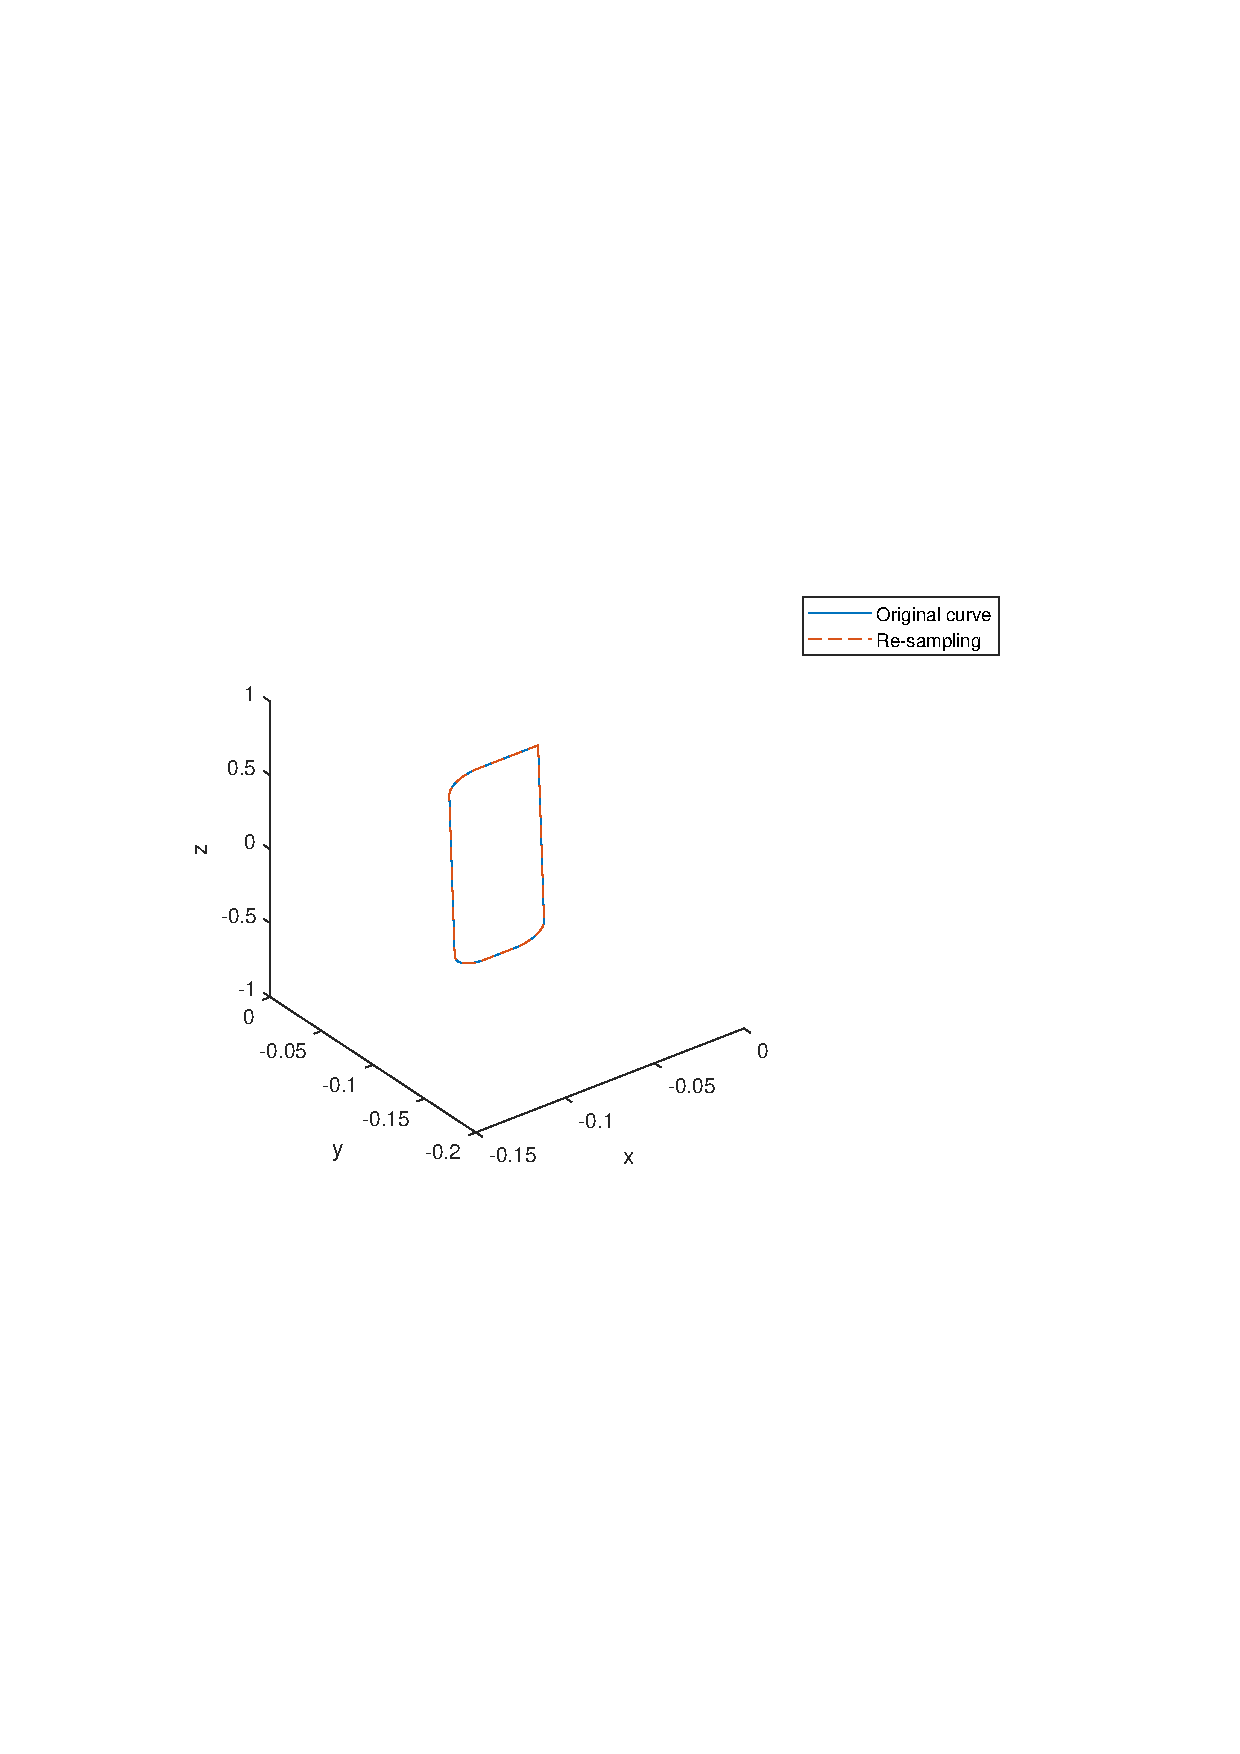
\includegraphics[width=\textwidth]{03_images/sample_point.pdf}
% 	\caption{Comparison of original and resampling curves}
% 	\label{fig:main:samplepoints}
% \end{figure}
\section{Physically couppled robot} \label{sec:scheme:robot}
